%.-------------------------------------------------------------------------------------------------------------------------------------------------------------
The DD is thought to guarantee that the components of the system are able to enforce the requirements presented in the RASD.
\newline
In this Chapter we show which components communicates with each other to enforce the fulfillment of the requirements.
\subsection{Requirements and system interactions}
A small description of the interactions is here to show how the communication should be performed.  
\begin{itemize}
\item R1) Authorities’ location must be known by the system when they are in service: Authority Position Servlet gets data about authorities' location and through User Manager, the  application sends data to the server everytime the authority moves from the previous locationn of at least more than 200 meters.
\item R2) When a Citizen makes a report the position is correctly added with the GPS when is available: Mobile application communicates with the GPS component of the Mobile phone , if available, to retrieve the position.
\item R3) The right authorities are notified about violations : Notification Manager gets Authority position from database. The position is updated by User Manager which communicates with the DataBase Connection package trough DataAccess Facade.
\item R4) Authority must be able to provide the system how the assignment finished, resolved and the
type of violation, no intervention needed when arrived, false report: Application after an authority accepted an assignment takes him/her to a screen where the assignment can be terminated.
This Screen allows user to communicate with the Assignment Servlet which notifies the Report Manager.
\item R5) The system must make Statistics available when asked:Data Access Facade allows all manager classes in the server package to access data which can be showed to users. User may query data making calls to the Statistics Manager
\item  R6) Statistics are always updated when an event happens: Report Manager allows the system to get new reports and also to terminate them, those data are stored in database using Data Access Facade and are used to build statistics
\item  R7) For registering a Municipality his/hers data must be provided to a System manager who will
add those data to the service to sign up him/her: web app allows user to insert all the needed data and doesn't allow to send data if all the needed data are not correctly inserted. For further security also Authority and municipality registration Servlet checks if all needed data are inserted.
\item  R8) A visitor must be able to begin sign up process in the SafeStreets App filling a form with his
data:when a visitor accesses to the SafeStreets mobile app the application shows him the Login page which contains the form to autenticate and the link to Sign upform and sends the data to the User Maanager.
\item  R9) When the creation of an account is successful the system must notify the Visitor sending an
email to the address provided in the sign up process: After inserting data of the user in the database the system sends an email, containing a corfimation message , to the user email through the Mail Manager.
\item  R10) When GPS is not available the user can input the position from a map: Mobile Application's interface provides the possibility to select a position on a map using Google Maps APIs.
\item  R11) Users to use the full service must be able to login providing the right credentials : User Manager Checks if inserted credentials are correct allowing user to access SafeStreets functionalities if they are correct.
\item  R12) The camera of the mobile phone must be accessible to take photos of violations: Mobile App implements the communication with the mobile phone's camera.
\item  R13) Suggestions must be available when municipalities requests them: Suggestion manager builds suggestions from data about violations, accidents but also static suggestions available on the database.
\item  R14) The User must be able to select the licence plate between the ones in output from the Licence
Plate Recognition algorithm :  Mobile Application's interface provides the possibility to select a Licence plate between the recognized ones.
\item  R15) Each Username is unique : User manager check the usernames during registration process. It doesn't allow different users to have the same username.
\end{itemize}
\clearpage
\subsection{Requirement Mapping with Server Managers}

\begin{figure}[H]
\centering
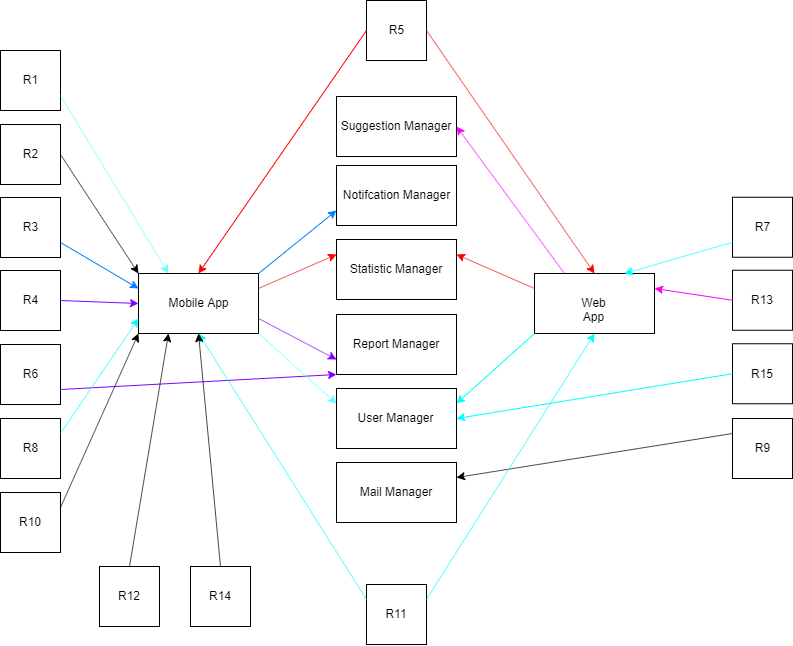
\includegraphics[width=\textwidth]{Images/ReqMapping.png}
\end{figure}
%.-------------------------------------------------------------------------------------------------------------------------------------------------------------
